\graphicspath{{chapt_dutch/}{intro/}{conclusions/}}

% Header
\renewcommand\evenpagerightmark{{\scshape\small Chapter 7}}
\renewcommand\oddpageleftmark{{\scshape\small Conclusions \& Outlook}}

\hyphenation{}

\chapter{Conclusions \& Outlook}

\begin{flushleft} 
\textit{This is the way the world ends\\
Not with a bang but a whimper.}
\end{flushleft}
\begin{flushright}
-- T.S. Eliot, \textit{The Hollow Men}
\end{flushright}

One of the remaining unsolved mysteries in the universe is the presumed existence of dark matter. Various astrophysical observations indicate the presence of an unknown type of matter next to the known visible matter. As it does not interact electromagnetically, only very little is know about this new type of matter, and many theories exist to explain its nature and origin. These theories can be tested through a variety of techniques and experiments. Depending on the exact nature of the dark matter particles, they could also be produced at colliders in high-energy collisions between Standard Model particles. Currently, the largest particle accelerator in the world is the \ac{LHC} at \ac{CERN}, which provides proton-proton collisions with a record centre-of-mass energy of \SI{13}{TeV} at a very high rate. In this thesis, two complementary searches for dark matter have been performed with data collected by the \ac{CMS} detector located at one of the interaction points of this collider.

% \section{Conclusions}

For both analyses, simplified model interpretations were considered. While dark matter does not interact electromagnetically, in these models it is assumed to interact with the ordinary matter through a new force. In the first analysis, the dark matter candidates are expected to interact very weakly with Standard Model particles and leave the detector undetected. They can however be detected when they recoil against another object in the event. In this case, the studied signature is one or more jets together with missing transverse energy. This search was already performed during Run~1, and has now been improved for Run~2. One of the main developments was the refinement of the prediction of events with a $Z$ boson decaying to two neutrinos in association with one or more jets, which led to an improved sensitivity. While the first iteration of this analysis with Run~2 data sets less stringent limits on the scenario with a vector mediator compared to the Run~1 analysis, the new results including the discussed improvements and using data corresponding to $12.9\ \mathrm{fb}^{-1}$ set stronger limits up to mediator masses of \SI{1.95}{TeV}. Similar results are obtained for an axial-vector mediator. Scalar and pseudoscalar mediator masses are excluded up to \SI{100}{GeV} and \SI{430}{GeV}, respectively.

% Why limits with ALL 2016 data not better than 12.9/fb?

In the second analysis, a different simplified model is considered, where the dark matter particles are assumed to interact strongly with Standard Model particles, through a new, light mediator. The produced pair of stable, neutral dark matter candidates will then give a signature consisting of a pair of trackless jets. First, a feasibility study for this model and corresponding signature was performed and published. For this study, the analysis strategy was developed, and the achievable sensitivity was investigated. This model had never been tested at colliders before, and as the feasibility study showed promising results, this signature was now studied for the first time at \ac{CMS} in this analysis, using a type of jets that is typically rejected by the jet identification criteria. While this search is very sensitive to new physics and the expected background was very efficiently reduced, some complications emerged as well. As an example, care was taken to account for the possibility of a wrongly chosen primary vertex, as this problem in the reconstruction can mimic signal-like events. A different issue was related to data taking and originated from the tracker APV pre-amplifier saturation problem, which occurred during the first half of the 2016 data taking period at \ac{CMS}. Due to the nature of this issue, the data affected by this problem were rejected for the analysis, and data corresponding to a total of $16.1\ \mathrm{fb}^{-1}$ were used. Moreover, the photon veto, which is crucial to reject background events coming from the production of a photon and a jet, was extended to take into account photon conversions as well. The outcome of this analysis yielded no observation of new physics, and all the considered dark matter masses, from \SI{1}{GeV} up to \SI{1}{TeV}, were excluded. Additionally, model-independent limits were derived as well, excluding production cross sections down to \SI{0.18}{fb}.

Both results can be translated into limits on the dark matter-nucleon interaction cross section, in order to compare the results with other experiments. Depending on the dark matter mass, the monojet analysis can exclude cross sections between approximately $10^{-6}\ \mathrm{fb}$ and \SI{0.1}{pb}, for the scalar or vector mediator case. In comparison, the trackless jets analysis excludes interaction cross sections of about $1-10\ \mathrm{mb}$, thus complementing the monojet results at higher cross sections.

% \section{Outlook}

In the future, the monojet analysis will be able to cover a larger part of phase space, going to higher mediator and dark matter masses. Projections can for example be made for the expected sensitivity at the high luminosity \ac{LHC}, which is expected to deliver $3000\ \mathrm{fb}^{-1}$ of integrated luminosity at a centre-of-mass energy of \SI{14}{TeV}. The expected reach is shown in Figure~\ref{fig:monojet_HLLHC} for an axial-vector and pseudoscalar mediator. 
% For the study involving an axial-vector mediator, the binning in missing transverse momentum binning was extended to optimise the sensitivity, and three scenarios were considered for the systematic uncertainties. 
The nominal scenario assumes that the level of control of the $E_T^{miss}$ distribution will remain the same as in the current analysis. Two more scenarios are shown, where the systematic uncertainties are reduced by a factor 2 and 4. 

For the pseudoscalar mediator, 
% the same binning in $E_T^{miss}$ was kept and the systematic uncertainties were extrapolated. At low missing transverse momentum, 
the systematic uncertainties are dominated by the uncertainty on lepton identification and isolation efficiencies used in the selection of events in the control regions at low missing transverse momentum. At high missing transverse momentum on the other hand, the systematic uncertainties are dominated by the statistical uncertainty. For the nominal scenario shown in the right plot of Figure~\ref{fig:monojet_HLLHC}, the systematic uncertainties are scaled by the luminosity at high $E_T^{miss}$ and scaled according to the predictions for the uncertainty on the lepton identification and isolation efficiencies at low $E_T^{miss}$. Additionally, a scenario is shown where the systematic uncertainties are reduced by a factor 2, as well as a scenario where the systematic uncertainties are scaled by the luminosity over the full $E_T^{miss}$ range.

\begin{figure}[ht]
  \centering
 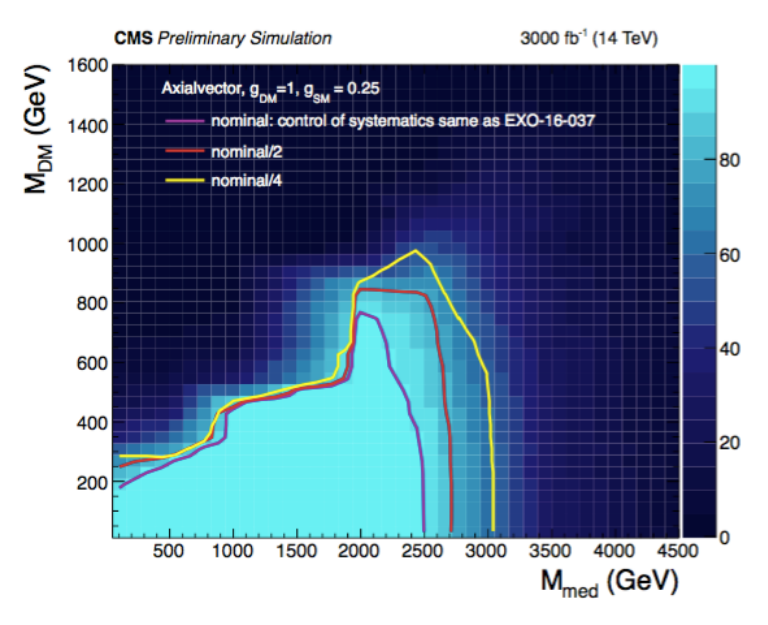
\includegraphics[width=.49\textwidth]{monojet_axial}
 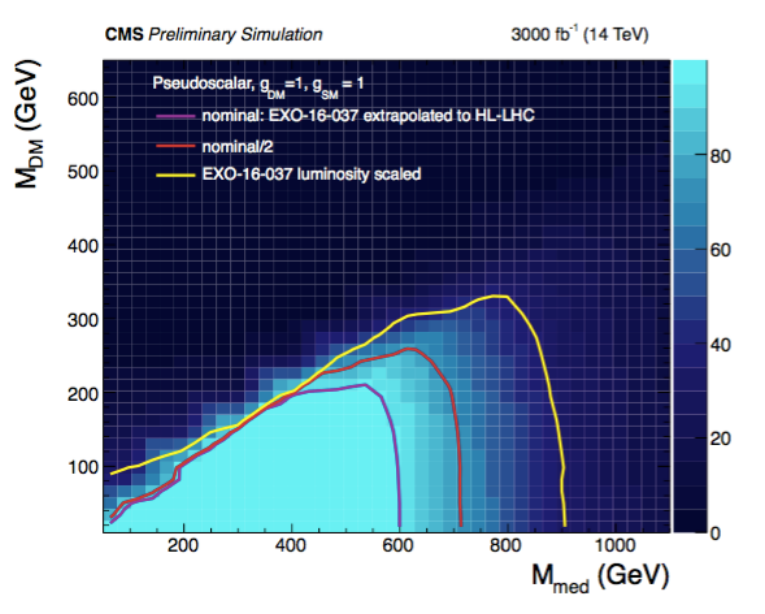
\includegraphics[width=.49\textwidth]{monojet_pseudoscalar}
 \caption{. Figures taken from~\cite{CMS-DP-2016-064}.}
 \label{fig:monojet_HLLHC}
\end{figure}

The obtained prospects show that mediator masses up to at least \SI{2.5}{TeV} and \SI{600}{GeV} could be excluded in the axial-vector and pseudoscalar case, respectively. This corresponds to an increase in range of about 30\%.

In the case of the trackless jets search, the entire considered dark matter mass range is already excluded by the described results. In a next step, the mass range could be extended, or the search could be broadened by allowing more extra jets, or including missing transverse energy in the signature. Alternative signatures can also be obtained by assuming a different interaction cross section, such as emerging jets or a cluster of tracks in the muon systems. Aside from \acp{SIMP}, Hidden Valley models can also give rise to this kind of signature. In these models, the interaction with the hidden sector can for example happen through rare Higgs boson decays. Additionally, trackless jets could also be produced by dark photons~\cite{Izaguirre:2015eya}. This model is now being studied as well, and the analysis can benefit from this first trackless jets analysis, among other things concerning the issue of the tracker APV pre-amplifier saturation. In the considered scenario, the neutral dark photon is produced in association with an ordinary photon. The resulting signature is then composed of a photon and a trackless jet with energy deposits in the \ac{ECAL} or \ac{HCAL}, or missing transverse energy, depending on the interaction strength. 

% trackless jets as QCD measurement?
% more info about Hidden Valleys? monojet: Higgs to invisible

%\renewcommand*{\thesection}{\thechapter.\arabic{section}}       % reset again to chaptnum.sectnum

\clearpage{\pagestyle{empty}\cleardoublepage}
